\documentclass{beamer}
\usetheme{Antibes}

\mode<presentation>

\title{Bayesian Phase Unwrapping with Factor Graphs}
\author{Eric Jonas}
\date{May 12, 2009}
\institute[6.556]{6.556 Final Project} 


\begin{document}

\begin{frame}
\maketitle
\end{frame}

\section{Phase Unwrapping for MR}
\begin{frame}

\end{frame}

\section{Factor Graphs and Markov Random Fields}
\begin{frame}
  \frametitle{Markov Random Fields}
  \begin{columns}
    \begin{column}{5cm}
      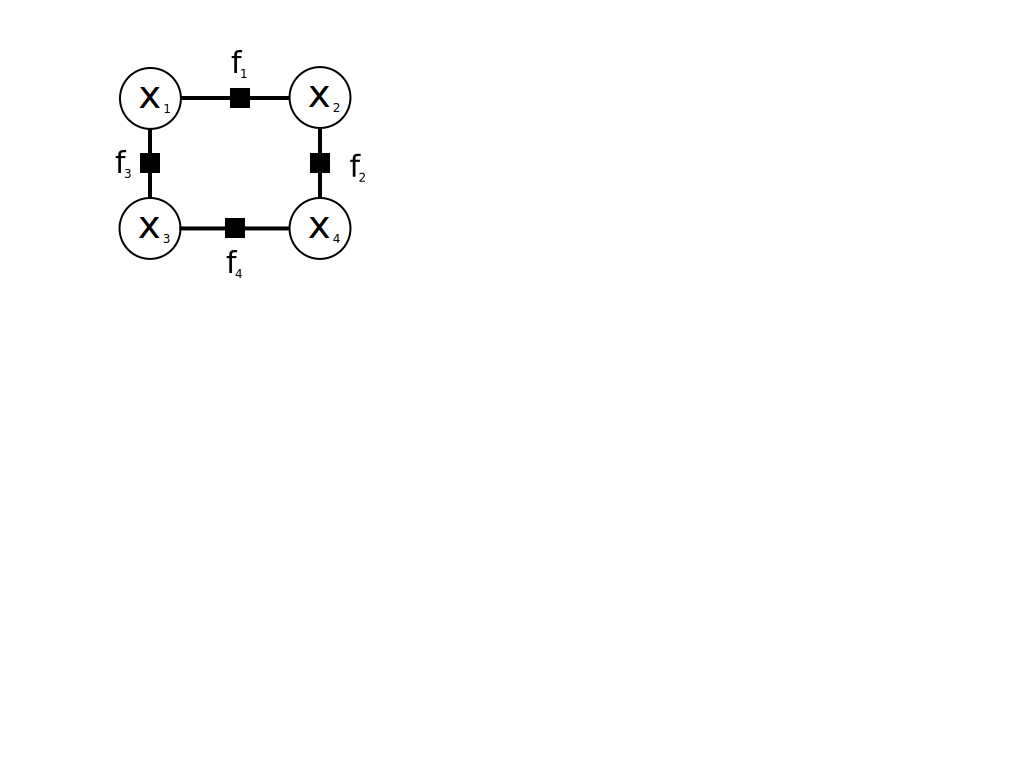
\includegraphics[width=1in]{4node_mrf.pdf}
    \end{column}
    \begin{column}{5cm}
      Markov random field, undirected graphical model, etc. 
    \end{column}
  \end{columns}
\end{frame}

\begin{frame}
  \frametitle{Factor Graphs}
  \begin{columns}
    \begin{column}{5cm}
      \includegraphics[width=4cm]{4node_fg.pdf}
    \end{column}
    \begin{column}{5cm}
      \begin{itemize}
        \item Factor Graphs \cite{Kschischang_Factor_01} express the same concepts
          as MRFs but make the \textbf{factors} explicit. 
        \end{itemize}
    \end{column}
  \end{columns}
  \begin{block}{Factor Graph Probability}
    \begin{equation}
      P(x_1, x_2, x_3, x_4) = f_1(x_1, x_2) \cdot f_2(x_2, x_3) \cdot f_3(x_3, x_4) \cdot f_4(x_4, x_1)
    \end{equation}
  \end{block}
\end{frame}

\begin{frame}
  \frametitle{Ising Model: The original lattice MRF}
  Imagine you want to simulate a spin system
  Statistical physics people love doing this

\end{frame}


\begin{frame} 
  \frametitle{Factor Graphs for Low-Level Vision}
  \begin{columns}
    \begin{column}{5cm}
      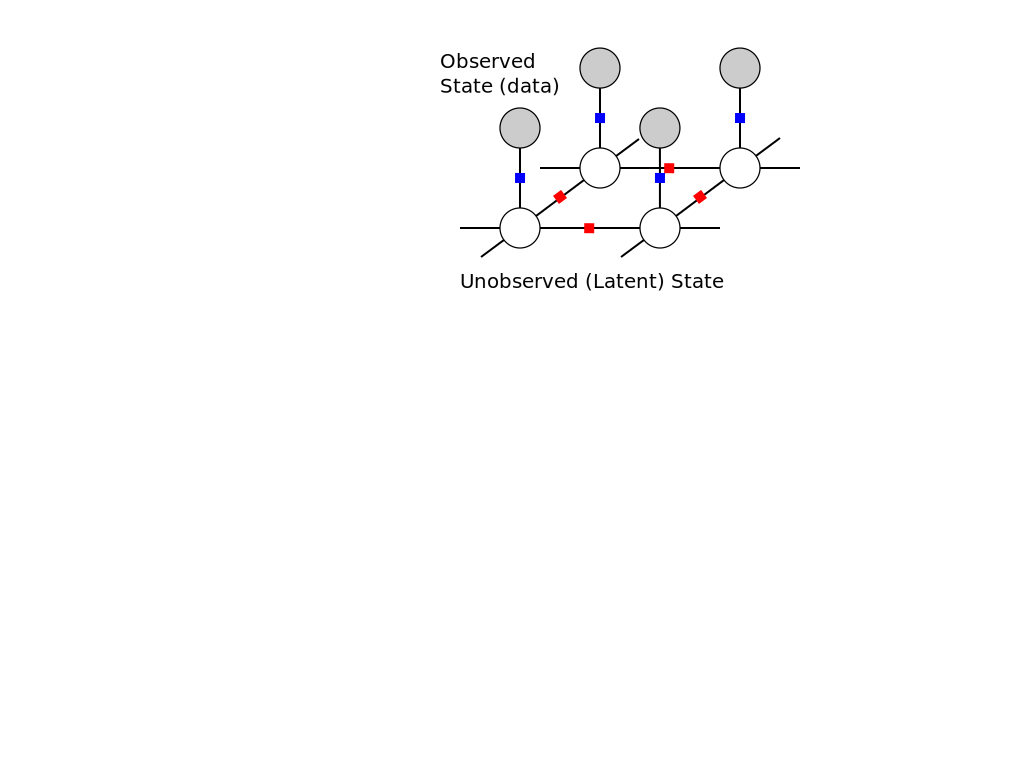
\includegraphics[width=6cm]{image_fg.pdf}
    \end{column}
    \begin{column}{5cm}
      Properties of Image Factor Graphs \cite{Freeman_Markov_1999}: 
      \begin{itemize}
      \item Use observed state (data) to infer hidden state
      \item Have lattice structure like the ising
      \item Large number of vertices ($O(n)$ in number of pixels)
      \item $O(1)$ per-vertex connectivity
      \item Typically have homogeneous factors
      \end{itemize}
    \end{column}
  \end{columns}
\end{frame}

\begin{frame}
\frametitle{Bayesian Factor Graphs}
\begin {columns}
  \begin{column}{5cm}
    \begin{block}{Bayes Rule} 
      \begin{equation*}
        P(X | Y ) = \frac{P(Y | X) P(X)}{\sum_XP(Y|X)P(X)}
      \end{equation*}
    \end{block}
  \end{column}
  \begin{column}{5cm}
    \begin{itemize}
    \item $Y = {y_{(i, j)}}$ : Observed Nodes
    \item $X = {x_{(bi, j)}}$ : Hidden state we wish to estimate
    \item $P(Y | X) $ : measurement model (``likelihood'')
    \item $P(X) $ : prior 
    \item 
    \end{itemize}
  \end{column}
\end{columns}
\end{frame}

\begin{frame}
\frametitle{Bayesian Factor Graphs For Low-Level vision}
Our factor graph gives us P(X, Y) 

\end{frame}

\subsection{MRFs for Phase Unwrapping}

\begin{frame} 
  \frametitle{MRFs for Phase: Frey's approach}
  In Ying and Frey's model \cite{Ying_Unwrapping_2006} they formulate 2-D phase
  unwrapping as a low-level vision MRF problem. 
  
  \begin{columns}
    \begin{column}{5cm}
      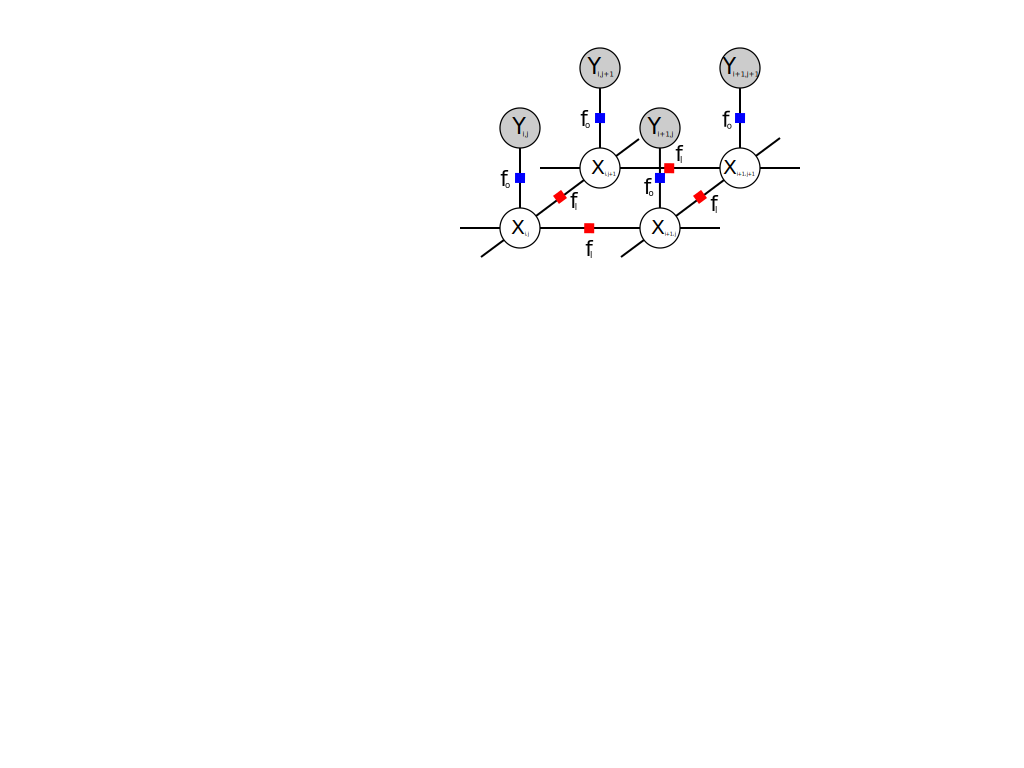
\includegraphics[width=5cm]{phase_fg_frey.pdf}
    \end{column}
    \begin{column}{5cm}
      \begin{itemize}
      \item $Y_{(i, j)} \in \mathbb{R}$
      \item $x_{(i, j)} \in [0, 2\pi)$
      \end{itemize}
    \end{column}
  \end{columns}
  
  
  \begin{columns}
    \begin{column}{5cm}
      \begin{block}{Observation Potential}
        \begin{equation*}
          f_o = \delta ((Y_{(i, j)}\mod 2\pi) - X_{(i, j)})
        \end{equation*}
      \end{block}
    \end{column}

    \begin{column}{5cm}
      \begin{block}{Latent potential} 
        \begin{equation*}
          f_l(X_1, X_2) = (X_1 - X_2)^2
        \end{equation*}
      \end{block}
    \end{column}
    
  \end{columns}
  
\end{frame}

\begin{frame}
  \frametitle{discrete latent state, uniform factors}
\end{frame}

\begin{frame}
\frametitle{discrete latent state, unique factors}
My formulation
\end{frame} 

\section{Inference in MRFs}

\begin{frame}
  \frametitle{Inference in MRFs}
  \begin{itemize}
  \item The MRF tells us how to compute $P(X, Y)$. Bayes rule
    tells us how to compute $P(X | Y)$. But the sum is awful. 
  \item But it's easy to compute $P^\ast(Y | X) $
  \end{itemize}
  Two generic approaches: 
  \begin{itemize}
  \item draw samples from $p(x | D)$ to empirically estimate 
  \item optimize to find MAP solution
  \end{itemize}
  \pause
  
  We focus on sampling (Why?) 
\end{frame}

\begin{frame}
  \frametitle{Markov-Chain Monte Carlo}
  Markov Property: next state only depends on current state
  \begin{equation*}
    p(x_{t+1} | x_{1:t} = p(x_{t+1} | x_{t})
  \end{equation*}

  Ergodic markov chains have stationary distributions
  
  Set up a state space so that the asymptotic limit is the target distribution

  Used in situations where you want to sample from
  $\pi(x)$ but only can compute $\pi^\ast(x)$

\end{frame}

\begin{frame}
  \frametitle{Metropolis Hastings}
  Consider a proposal distribution, $q(x \rightarrow x^\ast)$ 
  We draw $x^\ast$ as a \textit{new target state} from this distribution. 
  We compute the ``Acceptance'' ratio : 
  
  \begin{equation*}
    a = \min (1, \frac{p(x^\ast)}{p(x)} \cdot 
  \frac{q(x \rightarrow x^\ast)}{q(x^\ast \rightarrow x)})
  \end{equation*}

  %FIXME MH walk figure
  \cite{Metropolis_Equation_1953}
\end{frame}

\begin{frame}
  \frametitle{Gibbs Sampling}
  like MH but along an axis, useful when we can condition
  on other variables. 
  Look, we can Gibbs sample in image MRFs with discrete state spaces
  \cite{Geman_Stochastic_1990}
\end{frame}

\begin{frame}
  \frametitle{Parallel Tempering} 
  (aka ``Replica Exchange Monte Carlo'' \cite{Swendsen_Replica_1986}, aka ``Something to do with your 8 cores'')
  \begin{itemize}
  \item Run N replicas of your chain, each at a different temperature
  \item Periodically propose MH-style swaps between adjacent chains
  \item Let's hot chains move around in flatter energy landscape
  \end{itemize}
  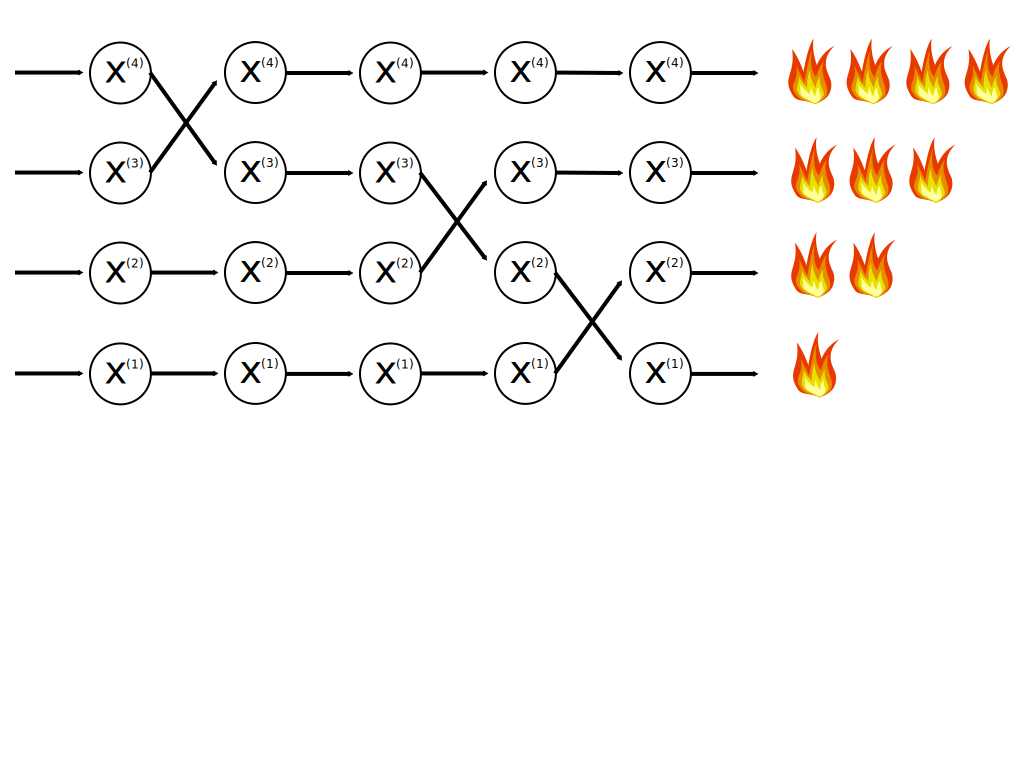
\includegraphics[width=8cm]{parallel_temp_fig.pdf}
\end{frame}

\begin{frame}
  \frametitle{Swendsen-Wang}
  Work Through
\end{frame}

\begin{frame}
  \frametitle{Data-driven MCMC}
  \begin{itemize}
    \item Any ``move'' is valid as long as it is reversable.  
    \item We can cheat a little bit and construct moves based on the data to help the chains mix, 
      without changing the target distribution
  \end{itemize}
  
  \cite{Tu_Image_2002}
  Work Through
\end{frame}

\begin{frame}
  \frametitle{Partial Replica Exchange}
  \cite{Liang_Evolutionary_2000}
\end{frame}

\begin{frame}
  \frametitle{MRFs and Parallelism}
  The conditional independence assumptions allow fine-grained parallelism
  
\end{frame}

\section{Our Implementation}
\begin{frame}
  \frametitle{Our Implementation}
  use SW, etc. 
  python, numpy, scipy, c++, boost, etc. 
  multithreaded
\end{frame}

\section{Performance}

How to measure performance? I'm going to go for 
log-likelihood, 

\subsection{Synthetic Data}
\begin{frame}
  \frametitle{2-D Synthetic Data}
\end{frame}

\begin{frame}
  \frametitle{3-D Synthetic Data}
\end{frame}

\subsection{Phantoms}

\subsection{Actual Data}
\begin{frame}
  \frametitle{Div and Audrey}
\end{frame}

\section{Methods Comparison}
\begin{frame}
  \frametitle{PRELUDE}
\end{frame}

\section{Concluson and Future Directions}
\begin{frame}
  \frametitle{Where to now?}
  Exact sampling using Systematic Stochsatic Search
  Better neighborhood connectivity / likelihood? 
  GPU implementation 
  Better visualization of posterior?
\end{frame}

\begin{frame}
  \frametitle{More information}
  Source is on github
  
\end{frame}

\end{document}
